% Biological analysis
\section{Emergent Transcription Factors in Biology} \label{s:N_I:sel_tfs_bio}

% Introduce the chapter
The analysis performed so far suggested that the 98 TF influence the stratification of the MIBC cohort, and in this part of the chapter, the role of the regulatory gene subset is explored in both the non-tumour\footnote{Remember non-tumour dataset is referred to throughout the project as the non-cancerous or healthy dataset. In all instances, it refers to the gene expression from the non-tumour samples in JBU; see \cref{s:lit:datasets_used}.} and tumour datasets.

It is worth remembering that MIBC is generally divided into Luminal and Basal subgroups. Compared with normal urothelial biology, the former exhibits a differentiated status and an undifferentiated status. The non-cancerous dataset contains differentiated (ABS-Ca or in situ) or undifferentiated samples. This implies that the TF with a high mean deviation may play a role in differentiation and help understand the Basal/Luminal dissimilarities in MIBC. The molecular particularities in the tissue types of differentiation tissues are next explored.

% Variance
\begin{figure}[!b]   
    \centering
    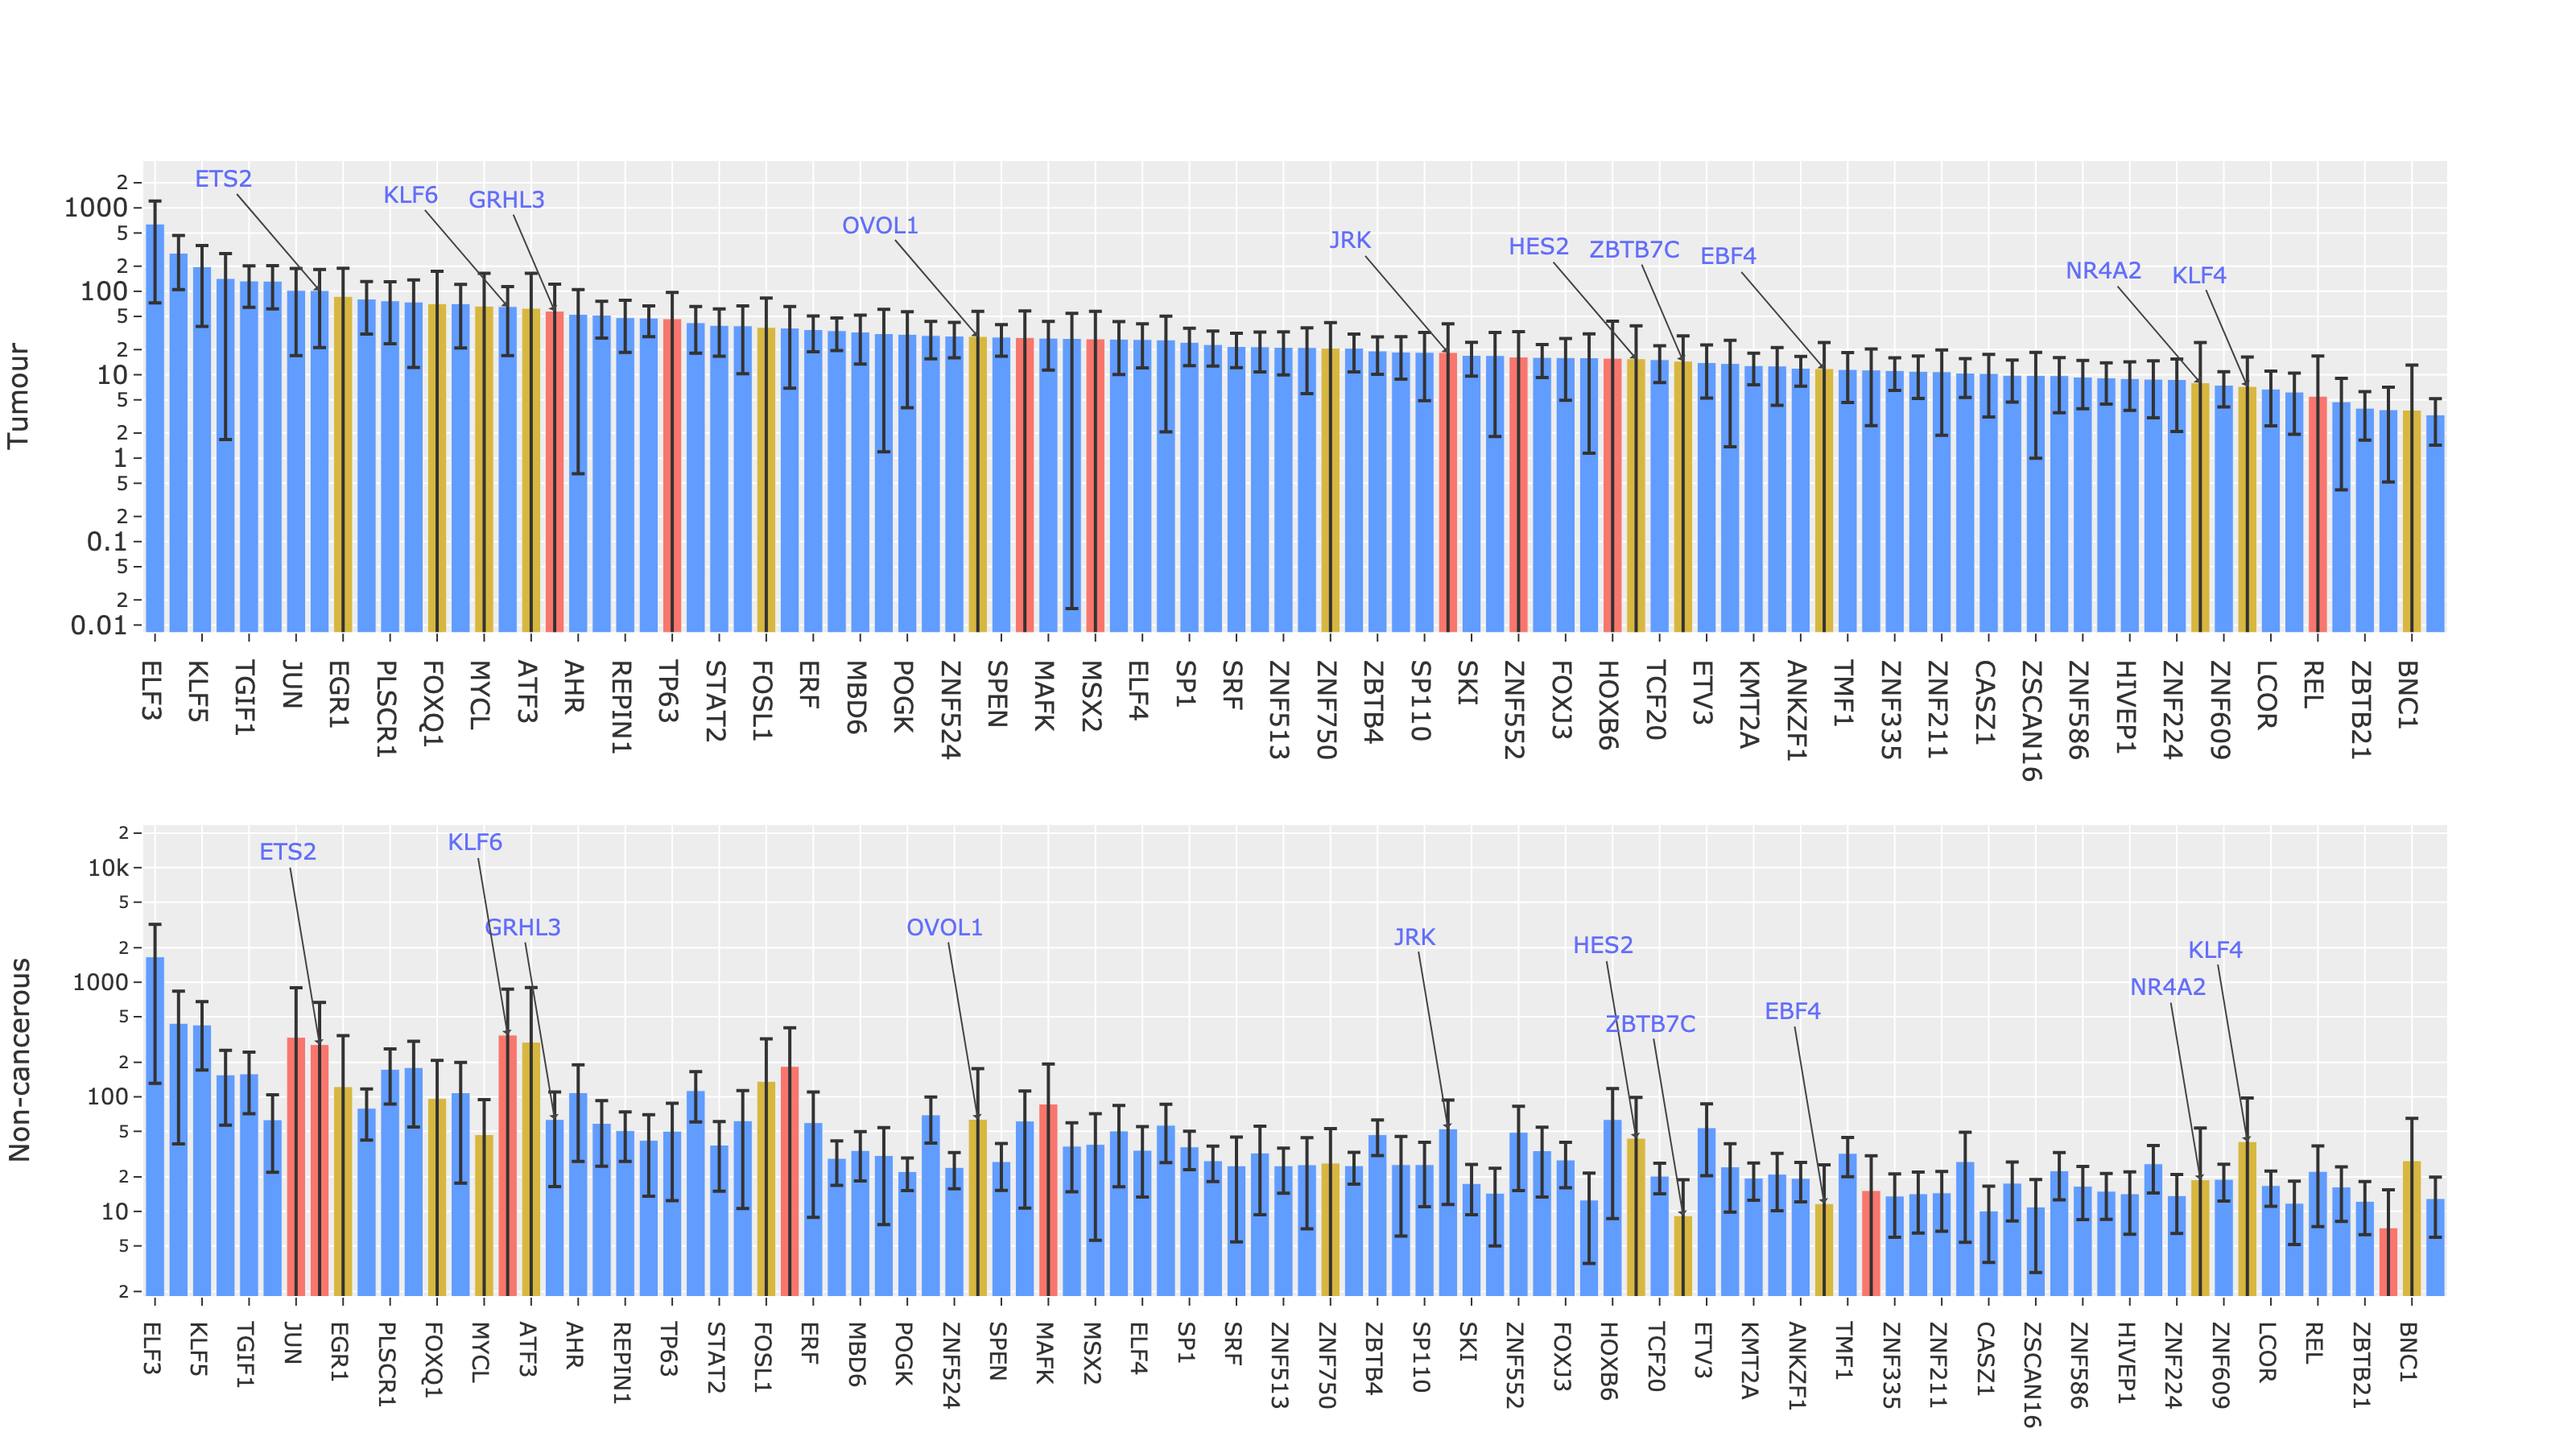
\includegraphics[width=1.0\textwidth,height=1.0\textheight,keepaspectratio]{Sections/Network_I/Resources/selective_pruning/sel_tfs/sel_tfs_var_tum_healthy.png}
      \caption[Mean expression of the 98 TF in tumour and healthy samples]{Bar plot of the log mean expression in both non-cancerous and tumour datasets with the error bars accounting for standard deviation. The genes are ordered in descending order by the mean values in the non-cancerous dataset. Red bars represents genes that have a high variance in the corresponding dataset, while the golden shows TFs appear in both tumour and non-cancerous datasets.}
    \label{fig:N_I:sel_tfs_var}
\end{figure}

% Introduce the plots
The bar plots in \cref{fig:N_I:sel_tfs_var} display the log mean of the gene expression in both non-cancerous and cancerous datasets of the 98 TF genes. The error bars depict the standard deviation of expression, and the genes are in the descending order of the tumour's average expressions. The red bars represent the genes with a high variance\footnote{In this case, a highly varied gene has a standard deviation as significant as the mean expression} in either the non-cancerous or tumour dataset, and the golden are the genes varied in both. Highly varied genes highlighted in the bar plot may yield important gene expression markers between the subgroups. The three lists of varied genes can be seen \cref{tab:N_I:sel_tfs_var}.


Variance in gene expression can indicate the potential genes specific to a group of samples. This means that \cref{fig:N_I:sel_tfs_var} helps to identify genes that might have an essential role in the two datasets used. A few genes are highly expressed in both the tumours and non-cancerous datasets, such as \textit{ELF3, KLF5} or \textit{JUN}. Later in the chapter, the analysis will show that genes like \textit{BHLHE41} or \textit{ZBTB7C} have the potential to be basal/luminal markers. A scatter plot version of the bar plot can be seen in \cref{fig:ap:sel_tfs_mean} from the Appendix, where the x-axis represents the non-cancerous mean, the y-axis the tum mean and the size and colour of the mutation burden of the genes.


\begin{table}[!t]
  \centering
  \small
  \begin{tabularx}{\textwidth}{>{\hsize=.25\hsize}X|>{\hsize=.75\hsize}X}
    \toprule
    \textbf{Dataset} & \textbf{Genes} \\
    \midrule
    Varied in both datasets & \textit{OVOL1, FOSL1, KLF4, BNC1, MYCL, NR4A2, ZBTB7C, FOXQ1, ZNF750, EGR1, HES2, ATF3, EBF4} \\
    \midrule
    Tumours only & \textit{BHLHE41, JRK, MSX2, TP53, ZNF552, GRHL3, HOXB6, REL} \\
    \midrule
    Non-cancerous only & \textit{ZBTB10, ARID5B, KLF6, JUN, MAFF, ETS2, MAFK} \\
    \bottomrule
  \end{tabularx}
    \caption[Summary of the subset of 98 TF which are highly varied]{Gene selection from the 98 TF and in which dataset they vary. Variance is a an indicator for potential markers specific to a MIBC subgroup or bladder tissue differentiation marker.}
    \label{tab:N_I:sel_tfs_var}
\end{table}



% Undiff vs Diff
\subsection{Role in bladder differentiation} \label{s:N:sel_tf_diff_status}


To further understand the role of the 98 TF in the bladder tissue differentiation the Pi plot introduced in \cref{s:lit:pi} is used to explore the \gls{DEA} across three tissue differentiation datasets, shown in \cref{fig:N_I:pi_sel_tfs_var}. The pi values are computed using the DEA between the ABS-Ca differentiated and P0 (X-axis) and UD (Y-axis) samples. There are shown only the 98 TF found classified by their variance.

% Just the sel tfs - UD and P0
In \cref{fig:N_I:pi_sel_tfs_var}, it can be seen that \textit{BNC1} and \textit{HES2} are UD markers, which may also indicate specificity for squamous markers. \textit{TP53} is another squamous marker \citep{Robertson2017-mg}, but it is more significantly expressed in the UD over ABS-Ca comparison. \textit{FOSL1} is a highly varied gene that appears to be both an undifferentiated and P0 marker (note the difference in scale between the X-axis and Y-axis). \textit{KLF6} and \textit{JUN} are genes more specific to P0 but are also highly expressed in the undifferentiated tissue.

% Talk about the differentiation markers 
The two Y-positive quadrants contains the genes that are likely involved in the differentiation of the urothelium, closer to the x-axis, more specific to the culture mode, conversely to Y-axis to the P0. It is worth noting that most of the genes specific to ABS-Ca model are highly varied in the tumours, which may suggest that are more expressed in the Luminal tumours compared to the Basal; \textit{HOXB6, ZNF552, JRK, BHLHe41}; quadrant I. Genes \textit{ZBTB7C, MSX2, MYCL, GRHL3 and REL} are specific to both P0 and ABS-Ca shown in quadrant IV. Both \textit{MYCL, GRHL3} are known to be differentiation markers. There are also markers that are specific to P0 samples: \textit{EBF4, MAFK, ARID5B, EGR1, ETS2, MAFF, FOX1, KLF4, NR4A2, ATF3, OVOL1}. 

% Less of Undiferentiated markers
It can be noticed that there are several markers that might be UD specific (negative Y-axis) while some additional markers involved in differentiation which do not vary as much. The latter may suggest that these markers are common both in Basal and Luminal tumours. 

% No TF shared between UD and ABS-Ca
The samples from the ABS-Ca and UD datasets are at the opposite side of the differentiation spectrum, covered in \cref{s:lit:datasets_used}. This is supported by the Pi plot where there are are a few genes in quadrant II, the one present may indicate their role in the tissue differentiation. The points at the centre of the pi plot may indicate a list of TF that are at the core of bladder tissue, regardless of their differentiated status and if are freshly isolated samples or obtain in the \textit{in vitro} experiments.


\Cref{tab:N_I:markers_diff} summarises the TF classification based on the differentiation tissue type: ABSCa (differentiation in culture), P0 (differentiation in tissue) and undifferentiated (culture). The 'transitional' genes in ABSCa-UD, UD-P0 and P0-ABSCa may yield information about the common genes shared between differentiation tissue types.

% Summary table
\begin{table}[!htb]
  \centering
  \small
  \begin{tabularx}{\textwidth}{>{\hsize=.15\hsize}X|>{\hsize=.85\hsize}X}
    \toprule
    \textbf{Category} & \textbf{Genes} \\
    \midrule
    \textbf{P0} & \textit{KLF4, ETS2, PHF1, ARID5B, EGR1, FOXQ1, MAFF, JUNB, MAFK, NFIL3, SRF, RUNX1, CASZ1, ZBTB10, EBF4} \\
    \midrule
    \textbf{UD} & \textit{SLC2A4RG, ZXDB, SKI, TP53, ETS1} \\
    \midrule
    \textbf{AbsCa} & \textit{BCL6, MSX2, ELF3, GRHL3, REL, KLF5, ZNF552, SATB1, DBP, ETV7, ETV3, MECOM, REPIN1, SP1, ZNF586, ZBTB4, TEAD1, ATMIN, TMF1, SP100, FOXJ3, MBD1, STAT1, ANKZF1, IRF9, STAT2, NFATC4, ZNF224, ZSCAN16, JRK, BHLHE41, HOXB6} \\
    \midrule
    \textbf{AbsCa-UD} & \textit{BNC1, MSANTD3, HES2} \\
    \midrule
    \textbf{UD-P0} & \textit{KLF6, JUN, FOSL1, ERF, IRF6, KLF16} \\
    \midrule
    \textbf{P0-AbsCa} & \textit{NR4A2, ATF3, OVOL1, ZBTB7C, FOSL2, BCL6, MSX2, MYCL, ZNF750, ELF3, GRHL3, REL, KLF5, ZNF552, SATB1, DBP, ETV7, ETV3, MECOM, REPIN1, SP1, ZNF586} \\
    \bottomrule
  \end{tabularx}
  \caption[Tissue differentiation markers]{TF marker classified by being significantly expressed in the two DEA comparisons: P0 vs ABSCa and UD vs ABSCa in \cref{fig:N_I:pi_sel_tfs_var}.} 
  \label{tab:N_I:markers_diff}
\end{table}

\begin{sidewaysfigure}
    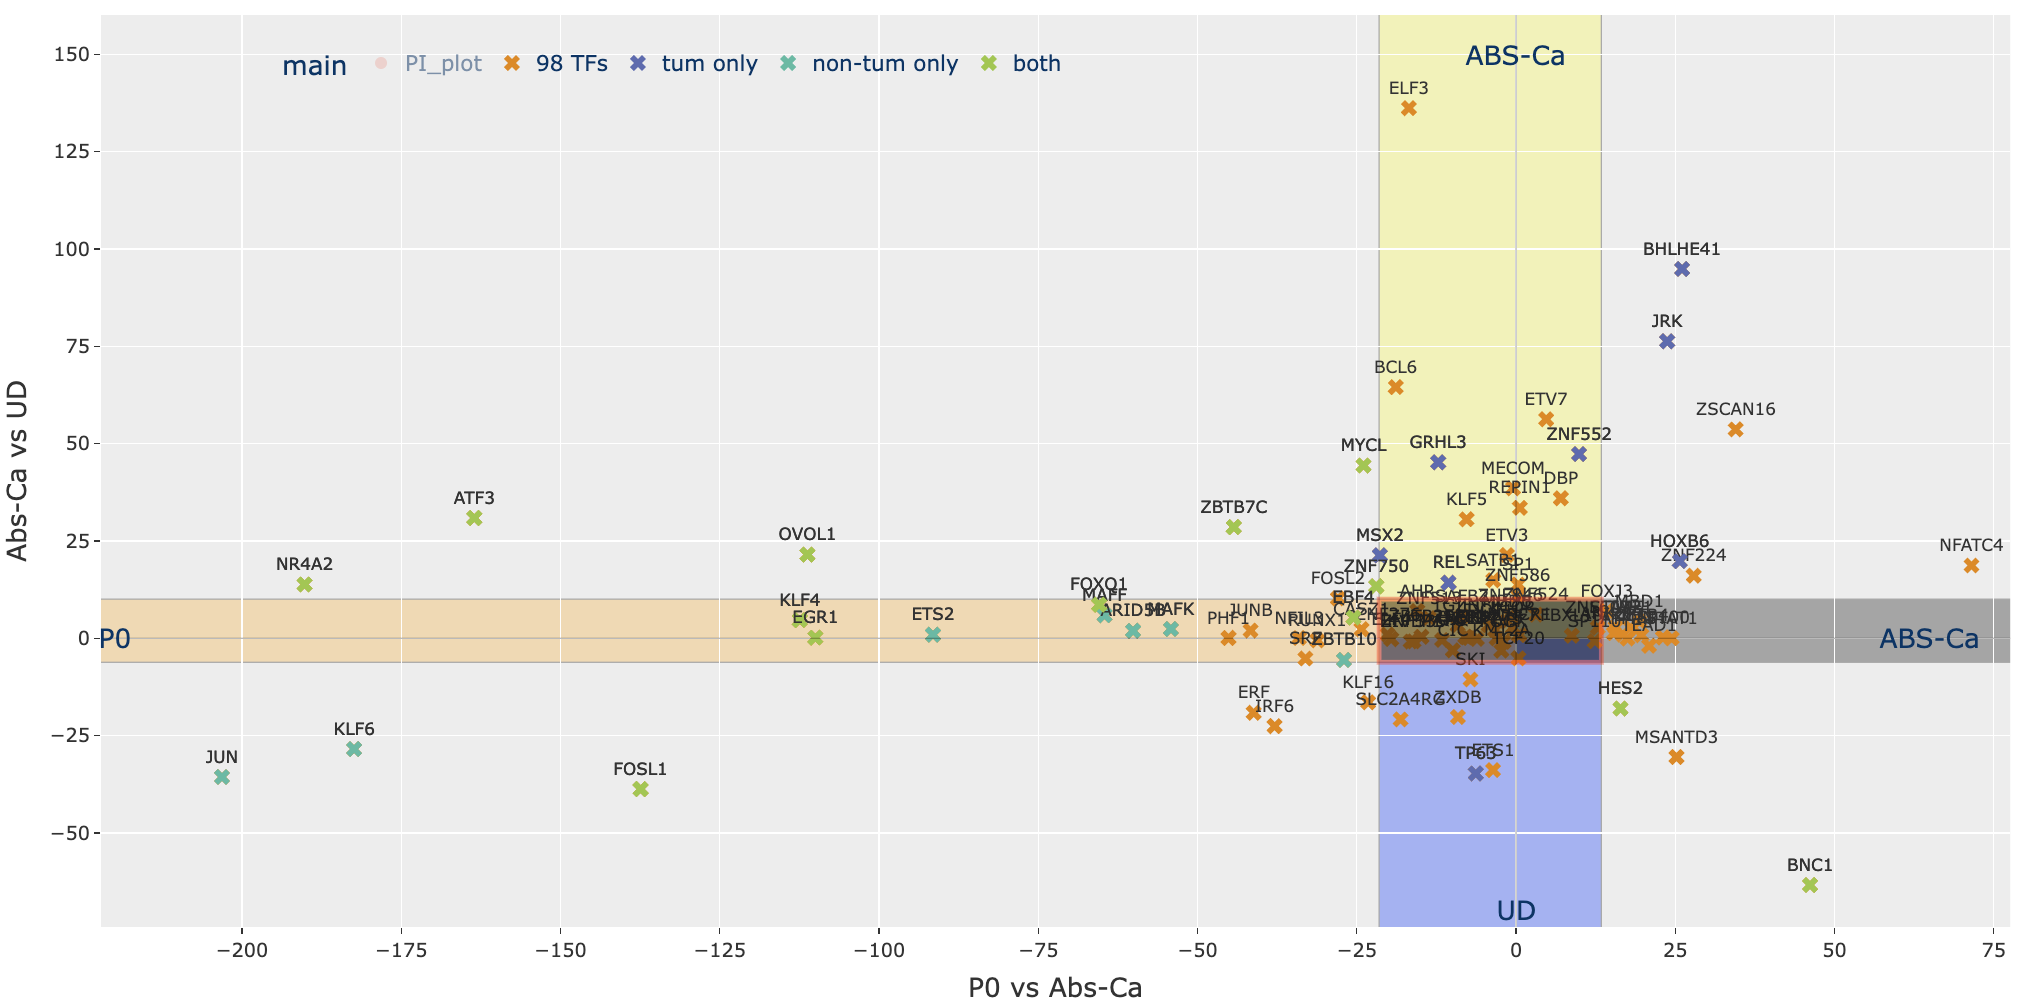
\includegraphics[width=1.0\textwidth,height=1.0\textheight,keepaspectratio]{Sections/Network_I/Resources/selective_pruning/sel_tfs/sel_tfs_pi_all_var_rect.png}
    \caption[The 98 TF and the DEA across the non-tumour datasets]{Pi plot across the three differentiation tissue types. The DEA is run between the ABS-Ca samples and the P0 (X-axis) and UD (Y-axis). Resulting in a scatter plot where the quadrants (Q) holds the genes specific to the ABS-Ca samples in Q I, ABS-Ca and UD in Q II, UD and P0 in Q III and P0 and ABS-Ca in Q IV. The markers in 
    are only varied in the tumour datasets, the blues only in non-tumour and yellow. the markers in red are genes TF that are core to the bladder cancer tissue. }
    \label{fig:N_I:pi_sel_tfs_var}
\end{sidewaysfigure}

\newpage


% Transitioning to cancer
\subsection{In muscle-invasive bladder cancer} \label{s:N_I:sel_tfs_cancer}


% Selecting the genes for basal and luminal, expression in both Basal and Luminal
The MIBC groups with luminal characteristics exhibit gene expression markers to differentiated bladder tumour which include ABS-Ca and freshly isolated samples, P0. The basal groups are molecular closer to the undifferentiated state of the urothelium. This means that the earlier devised TF markers for the three urothelium differentiation types can be also used to guide the the analysis for MIBC. In addition to these markers the box plots are used \cref{fig:N_I:box_basal_dendrogram,fig:N_I:box_luminal_dendrogram} to validate and determine the two lists of genes specific to Basal/Squamous (Ba/Sq) and Luminal subtypes  also shown in \cref{tab:N_I:genes_lum_basal}. 

% Comment on luminal differentiation
A recent study by \citet{Ramal2024-ha}, which investigated the regulatory network in urothelial cells, concluded that the following genes are considered 'novel putative TF' for luminal differentiation: \textit{\textbf{BHLHE41}, \textbf{MECOM}, \textbf{MYCL}, NCOA1, NR2F2, NR2F6, \textbf{REPIN1}, SREBF1, TBX2, TBX3, TRAFD1, and \textbf{ZBTB7C}}. The bold genes are among the 98 TF identified in this section, while \textit{MECOM, BHLHE41, ZBTB7C} are selected as markers in \cref{tab:N_I:genes_lum_basal}. \textit{GRHL3} is also mentioned in the work by \citet{Ramal2024-ha}, but it was already determined as a differentiation marker \citep{Bock2014-zy}. \citet{Chen2021-tc} studied the role of \textit{ZBTB7C} across different cancers and its relation to tumour mutational burden, micro-satellite instability, and immune cell infiltration. The genes in \textbf{bold} are in the luminal/basal markers derived and can be seen in \cref{fig:N_I:box_debdrogram,fig:ap:box_consensus} and in \cref{tab:N_I:genes_lum_basal}.

% Discuss Squamous work
\citet{Hurst2022-sp} researched the up-regulated and down-regulated genes involved in the formation of \acrfull{scc}, an undifferentiated tissue. Figure 4 from their paper shows the signature genes involved in this process. Among the up-regulated genes in \citet{Hurst2022-sp}, the following are found in the 98 TF: \textit{\textbf{BNC1}, EGR1, \textbf{FOSL1}, \textbf{HES2}, JUN, \textbf{KLF16}, KLF4, NFIL3}. From the list of down-regulated genes, the following are found in the 98 TF: \textit{\textbf{BHLHE41}, ELF3, FOXQ1, \textbf{MECOM}, POGK, REPIN1, ZSCAN16}. The genes in \textbf{bold} are in the luminal/basal markers derived and can be seen in \cref{fig:N_I:box_debdrogram,fig:ap:box_consensus} and in the table \cref{tab:N_I:genes_lum_basal}.

% 
Overall the analysis show that some of the 98 TF have a role in bladder cancer biology may represent new potential markers.

% Lum-basal markers
\begin{table}[!htb]
  \centering
  \small
  \begin{tabularx}{\textwidth}{>{\hsize=.25\hsize}X|>{\hsize=.75\hsize}X}
    \toprule
    \textbf{Category} & \textbf{Genes} \\
    \midrule
    \textbf{Luminal} & \textit{MSX2, HOXB6, MECOM, GRHL3, JRK, BHLHE41, ZBTB7C, ZSCAN16, ZNF224, ZBTB10} \\
    \midrule
    \textbf{Basal/Squamous} & \textit{TP53, BNC1, HES2, ERF, IRF6, ZXDB, ZNF750, ETS1, MSANTD3, FOSL1, KLF6, KLF16} \\
    \bottomrule
  \end{tabularx}
  \caption[Luminal and Basal markers from the 98 TF]{The 98 transcription factors markers categorised by Luminal and Basal subtypes.} % Caption for the table
  \label{tab:N_I:genes_lum_basal}
\end{table}


% Luminal/Basal Markers in the dendrogram cut
\begin{figure}[H]
    \centering
    % consensus
    \begin{subfigure}[!t]{1.0\textwidth}
        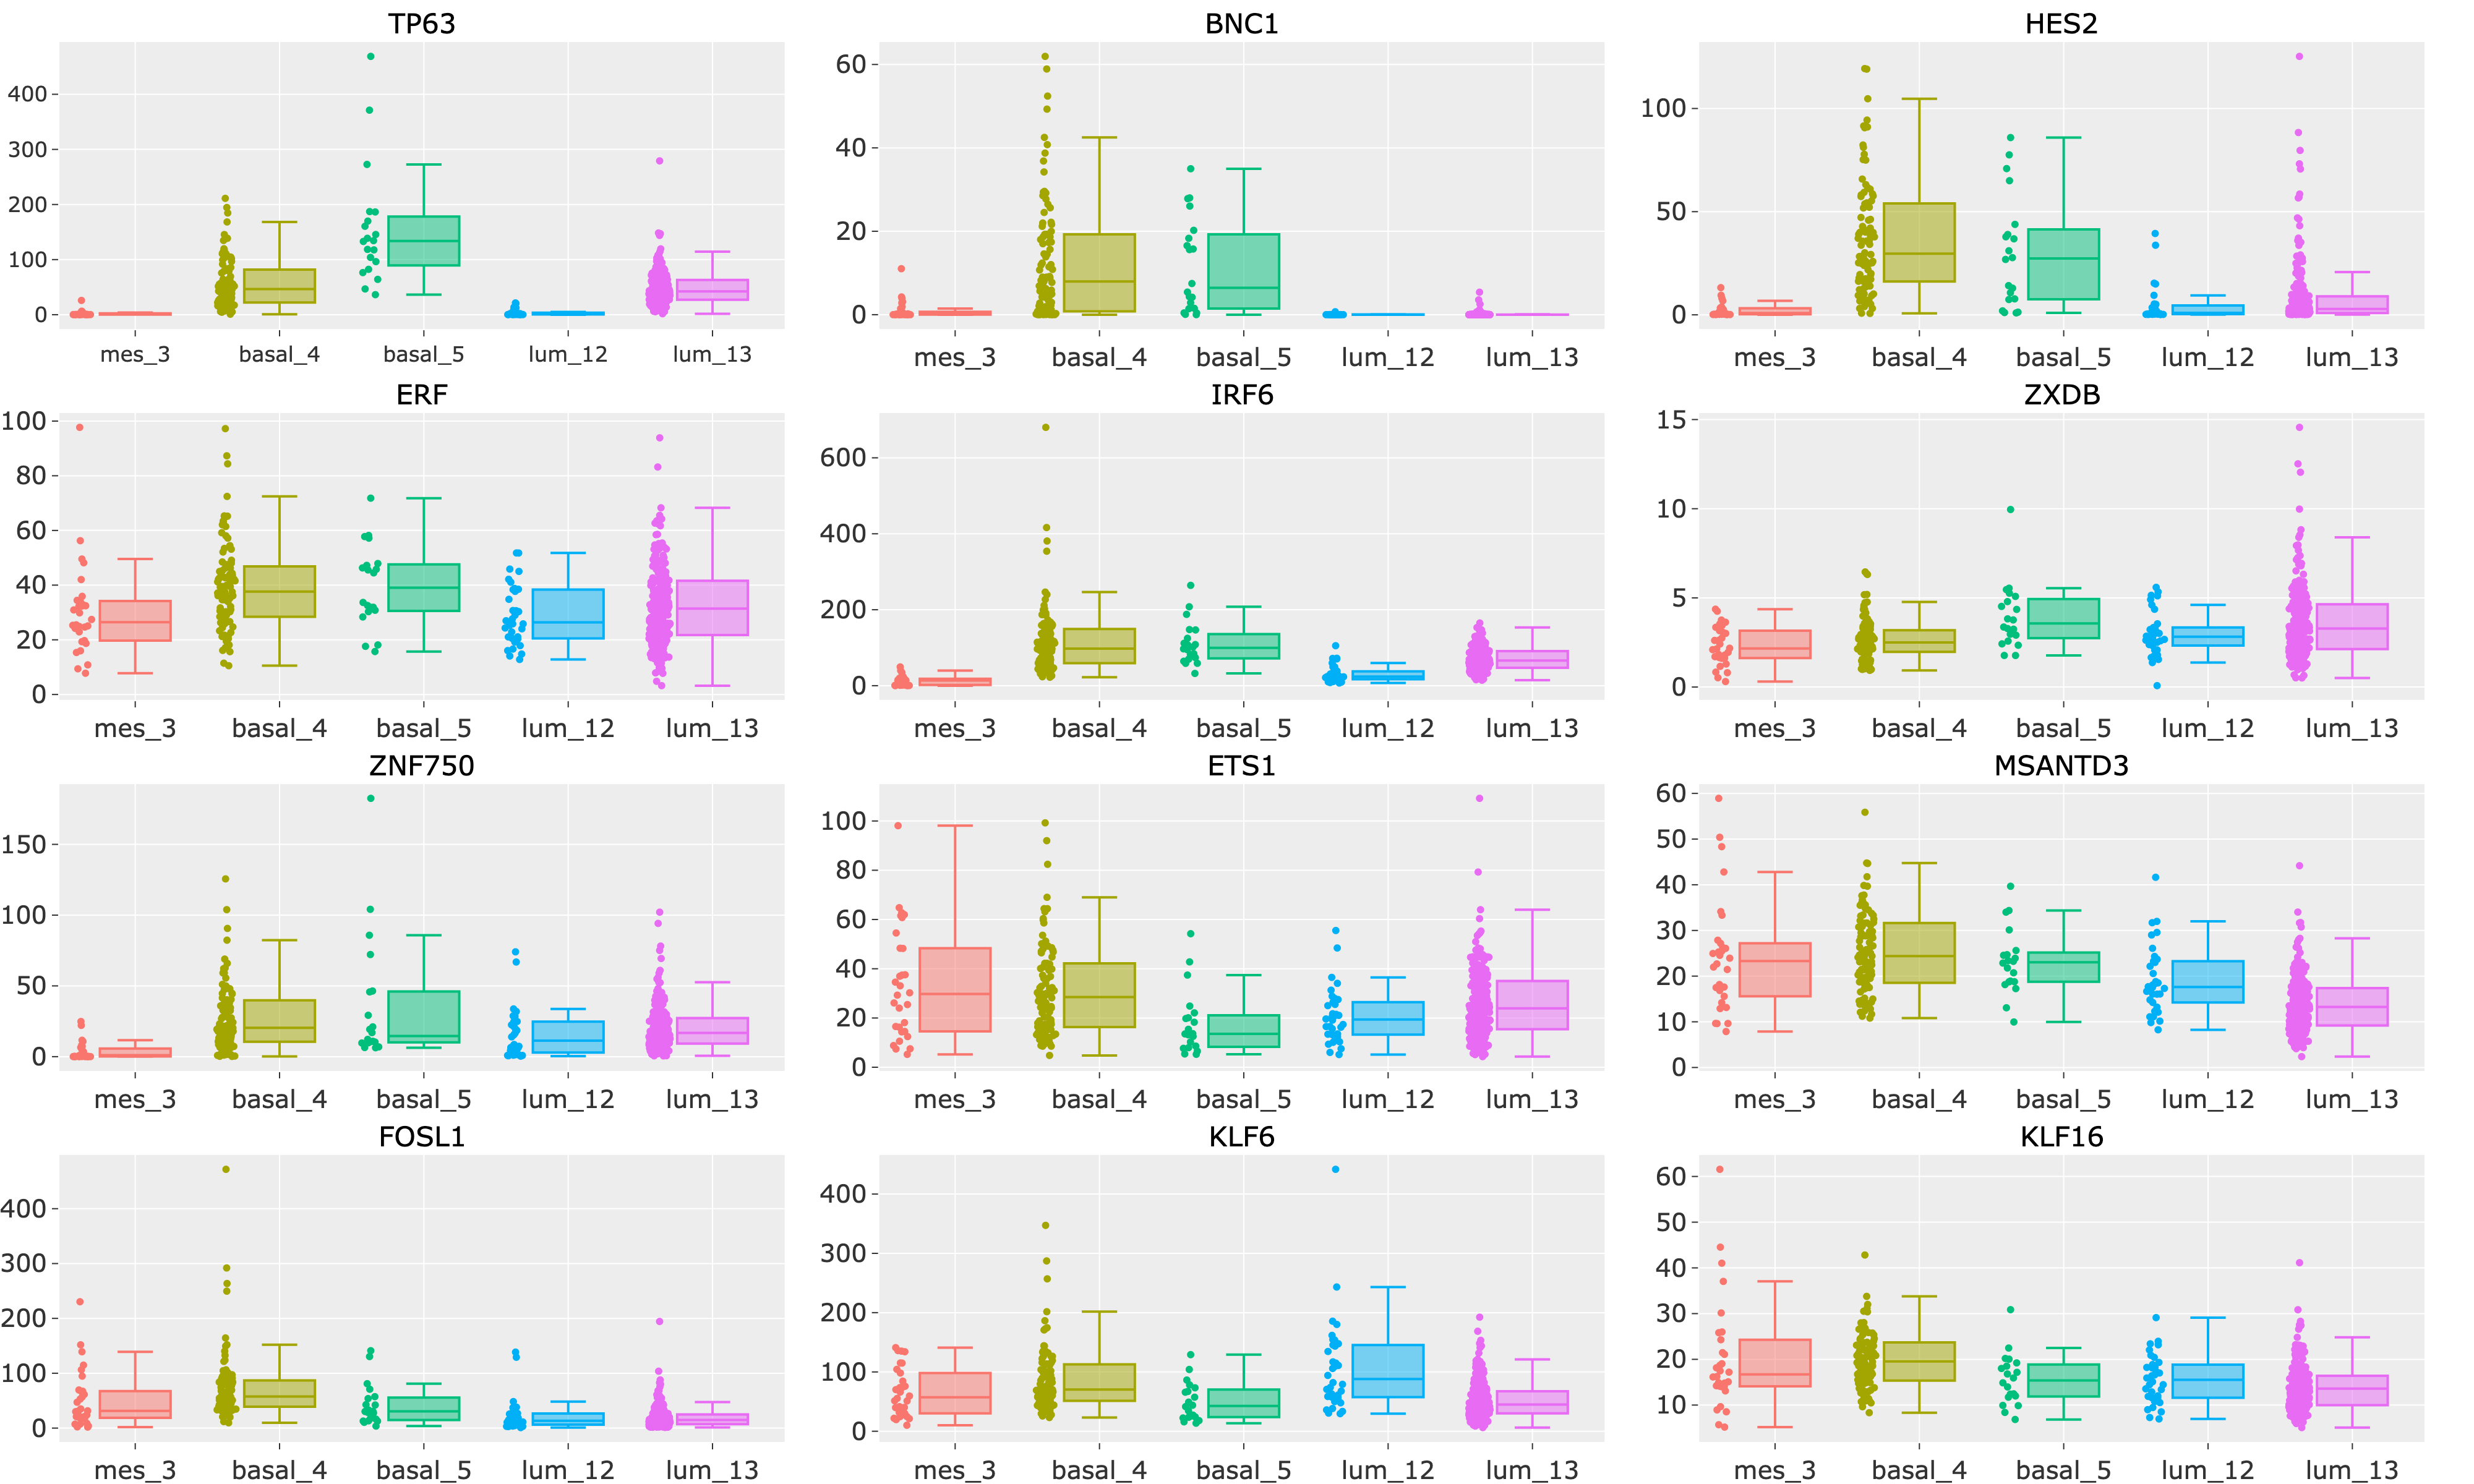
\includegraphics[width=1.0\textwidth,height=1.0\textheight,keepaspectratio]{Sections/Network_I/Resources/selective_pruning/box_plots/dendrogram_basal.png}
        \caption{Basal}
        \label{fig:N_I:box_basal_dendrogram}
    \end{subfigure}
    % dendrogram
    \begin{subfigure}[!t]{1.0\textwidth}
      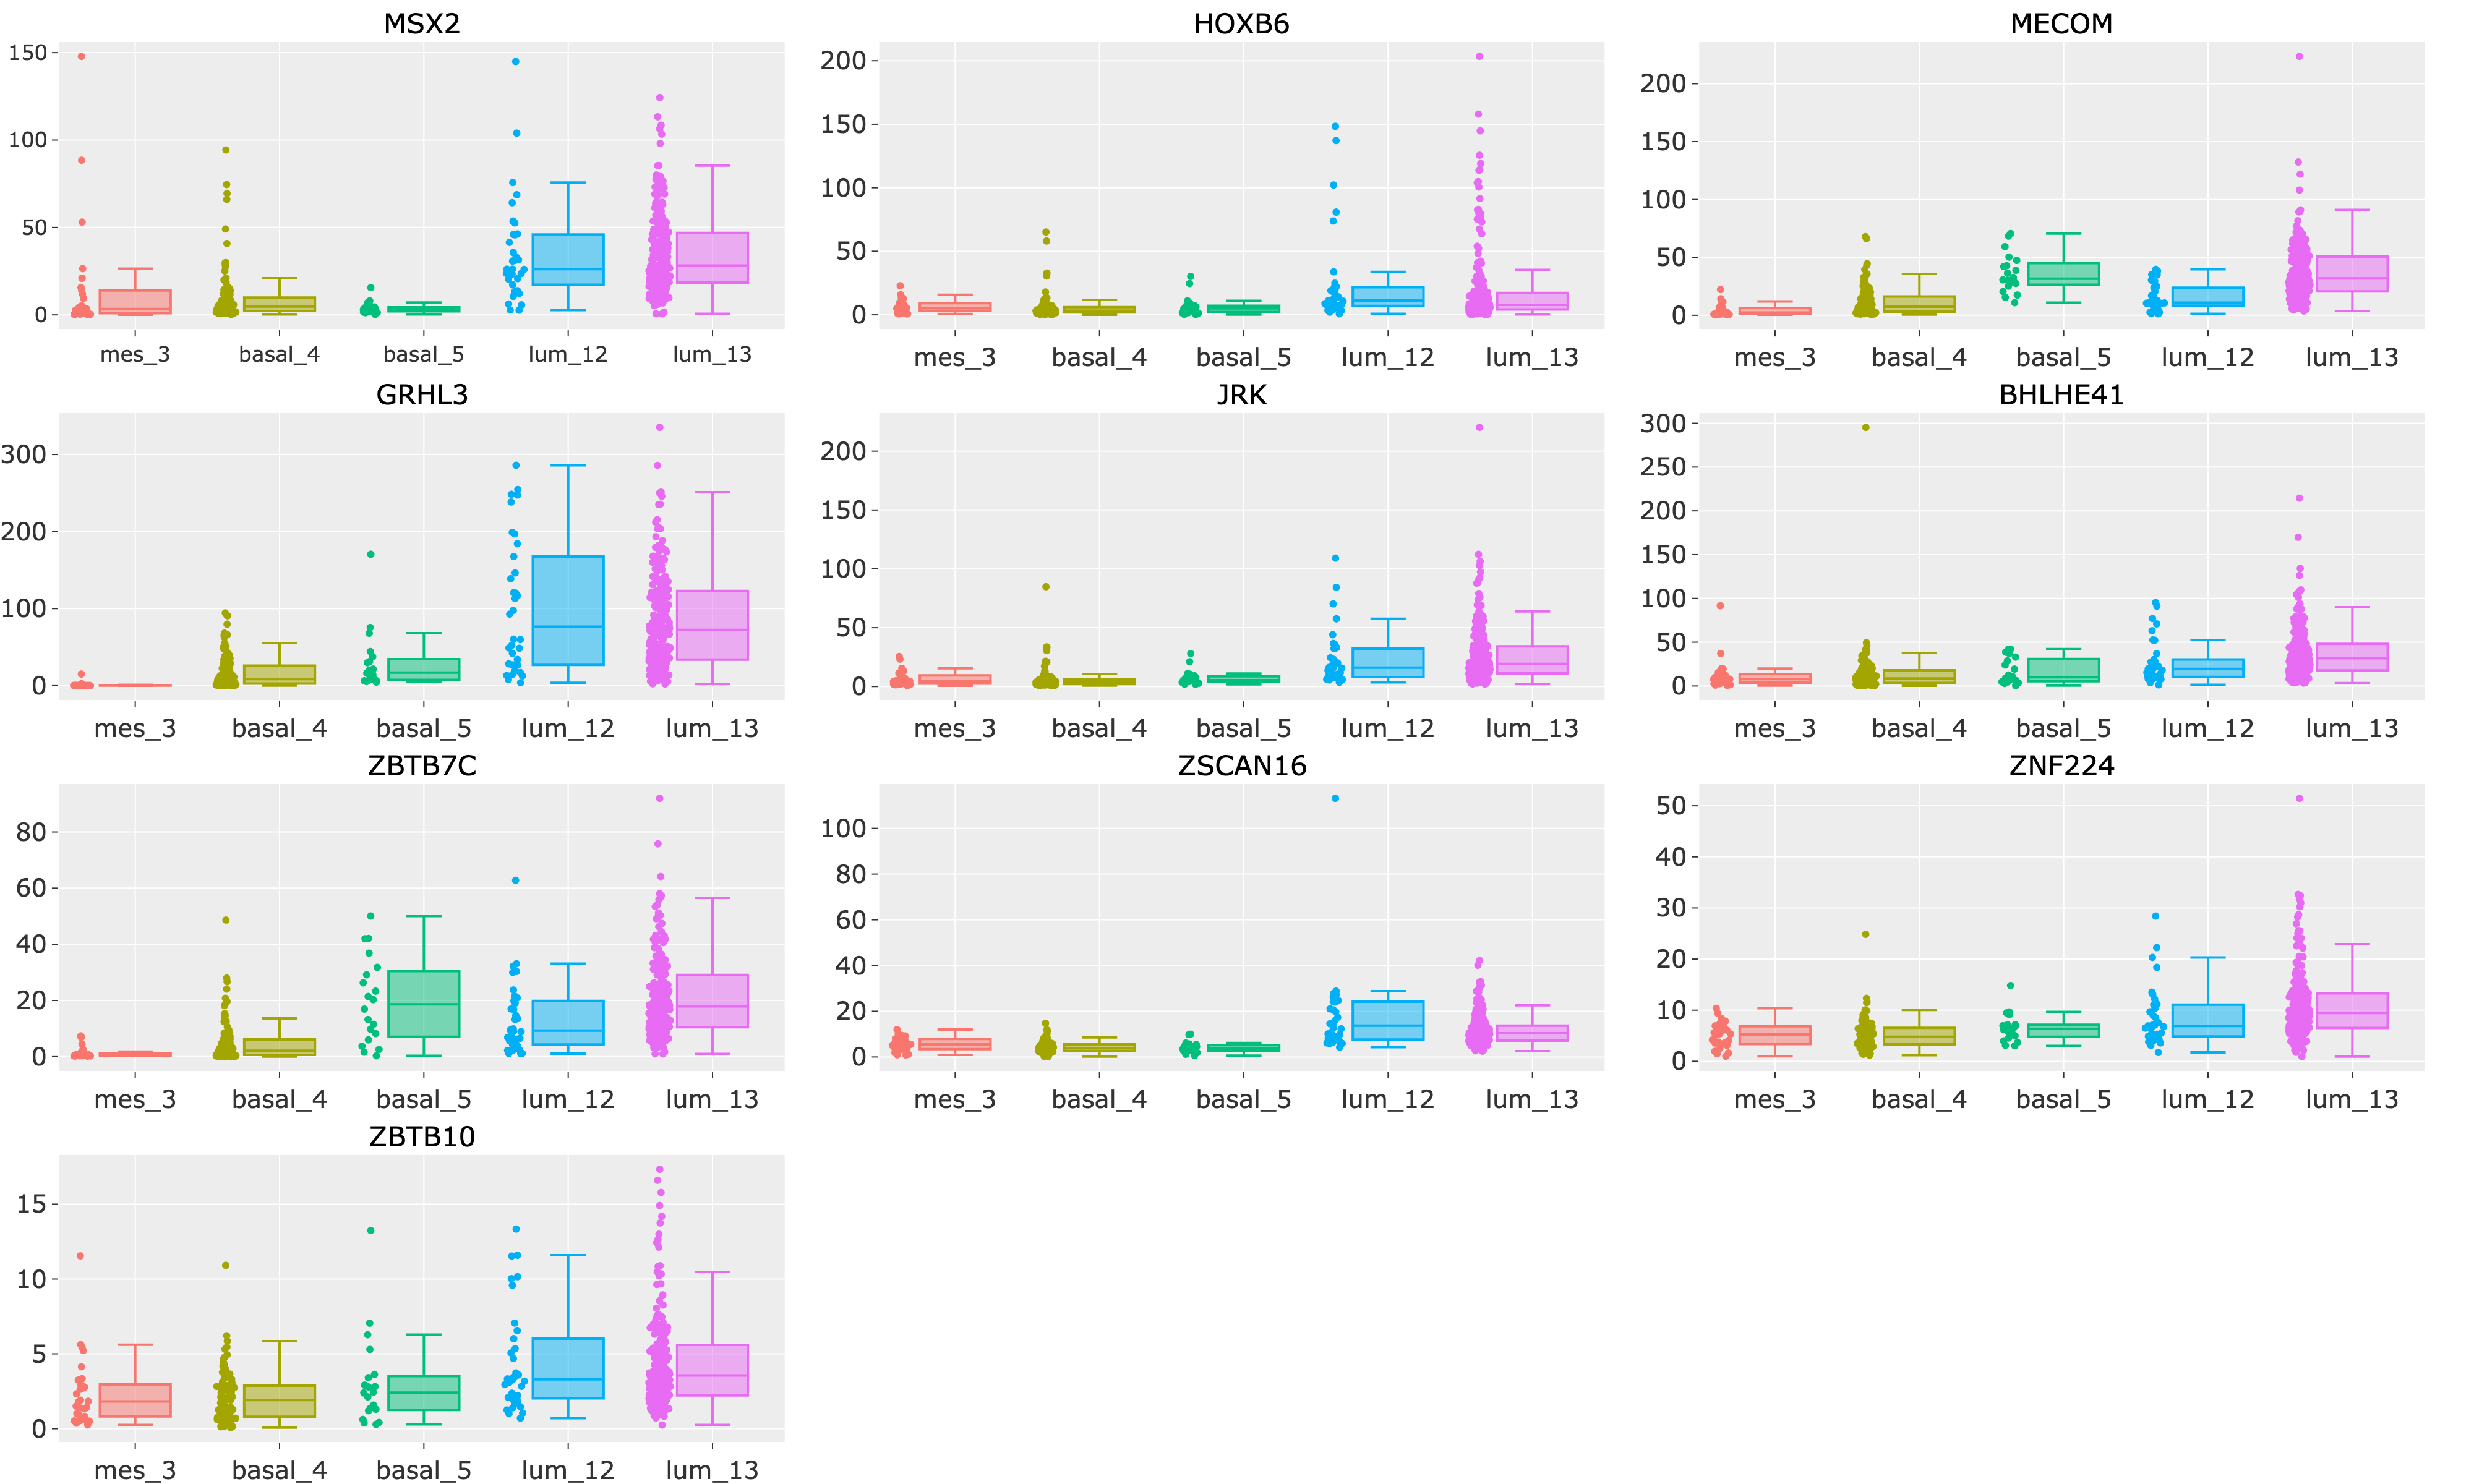
\includegraphics[width=1.0\textwidth,height=1.0\textheight,keepaspectratio]{Sections/Network_I/Resources/selective_pruning/box_plots/dendrogram_lum.png}
      \caption{Luminal}
      \label{fig:N_I:box_luminal_dendrogram}
    \end{subfigure}
    \caption[98 TF: expression of basal and luminal markers in the new groups]{Box plots showing the TPM spread of the \textbf{basal and luminal} markers over the MIBC groups derived using the 98 TF. A similar plot, \cref{fig:ap:box_consensus} was created with the two set of TF markers but for the consensus \citep{Kamoun2020-tj} subgroups in Appendix \cref{s:ap:sel_prun_markers}.}
    \label{fig:N_I:box_debdrogram}
\end{figure}



% Subtypes analysis
\subsection{Differentially expressed analysis} \label{s:N_I:sel_tfs_subtypes}

This section expands the analysis of the 98 TF and their impact on MIBC by performing \acrlong{dea}, followed by the use of a Pi plot to rank the genes for \acrfull{gsea}; methods introduced in \cref{s:lit:dea,s:lit:pi,s:lit:gsea}. For each of the five MIBC subtypes identified earlier—basal 3, basal 4, basal 5, luminal 13, and luminal 12—a Pi plot was created, which can be found in Appendix \cref{s:ap:sel_prun_pi}. 

It is important to note that the input data for GSEA across all subtypes uses the same list of genes but ranks them differently, prioritising genes specific to each studied subtype. As a result, the GSEA output includes pathways shared across the subtypes. To address this, the top ten \textbf{unique} pathways with the highest normalised enrichment score (NES) and a significant FDR q-value ($>$0.05) were retained for each MIBC group.

No unique signature was found for the mes 3 subgroup, as it shared several pathways with the basal 4 (e.g., interferon alpha and gamma pathways), as shown in the GSEA outputs in Appendix \cref{fig:ap:gsea_largeBasal,fig:ap:gsea_mesLike}.

The outputs of the GSEA runs using the Reactome database are summarised in two tables: one for the basal groups (\cref{tab:N_I:gsea_basal_reactome}) and another for the luminal groups (\cref{tab:N_I:gsea_luminal_reactome}). The top 10 terms, whether unique to the MIBC group or not, are listed in the Appendix \cref{s:ap:sel_tfs_gsea_reactome}.


% Basal 5
\subsubsection*{Basal 5}


% Pi plot for Small Ba/Sq
\begin{figure}[!htb]   
    \centering
    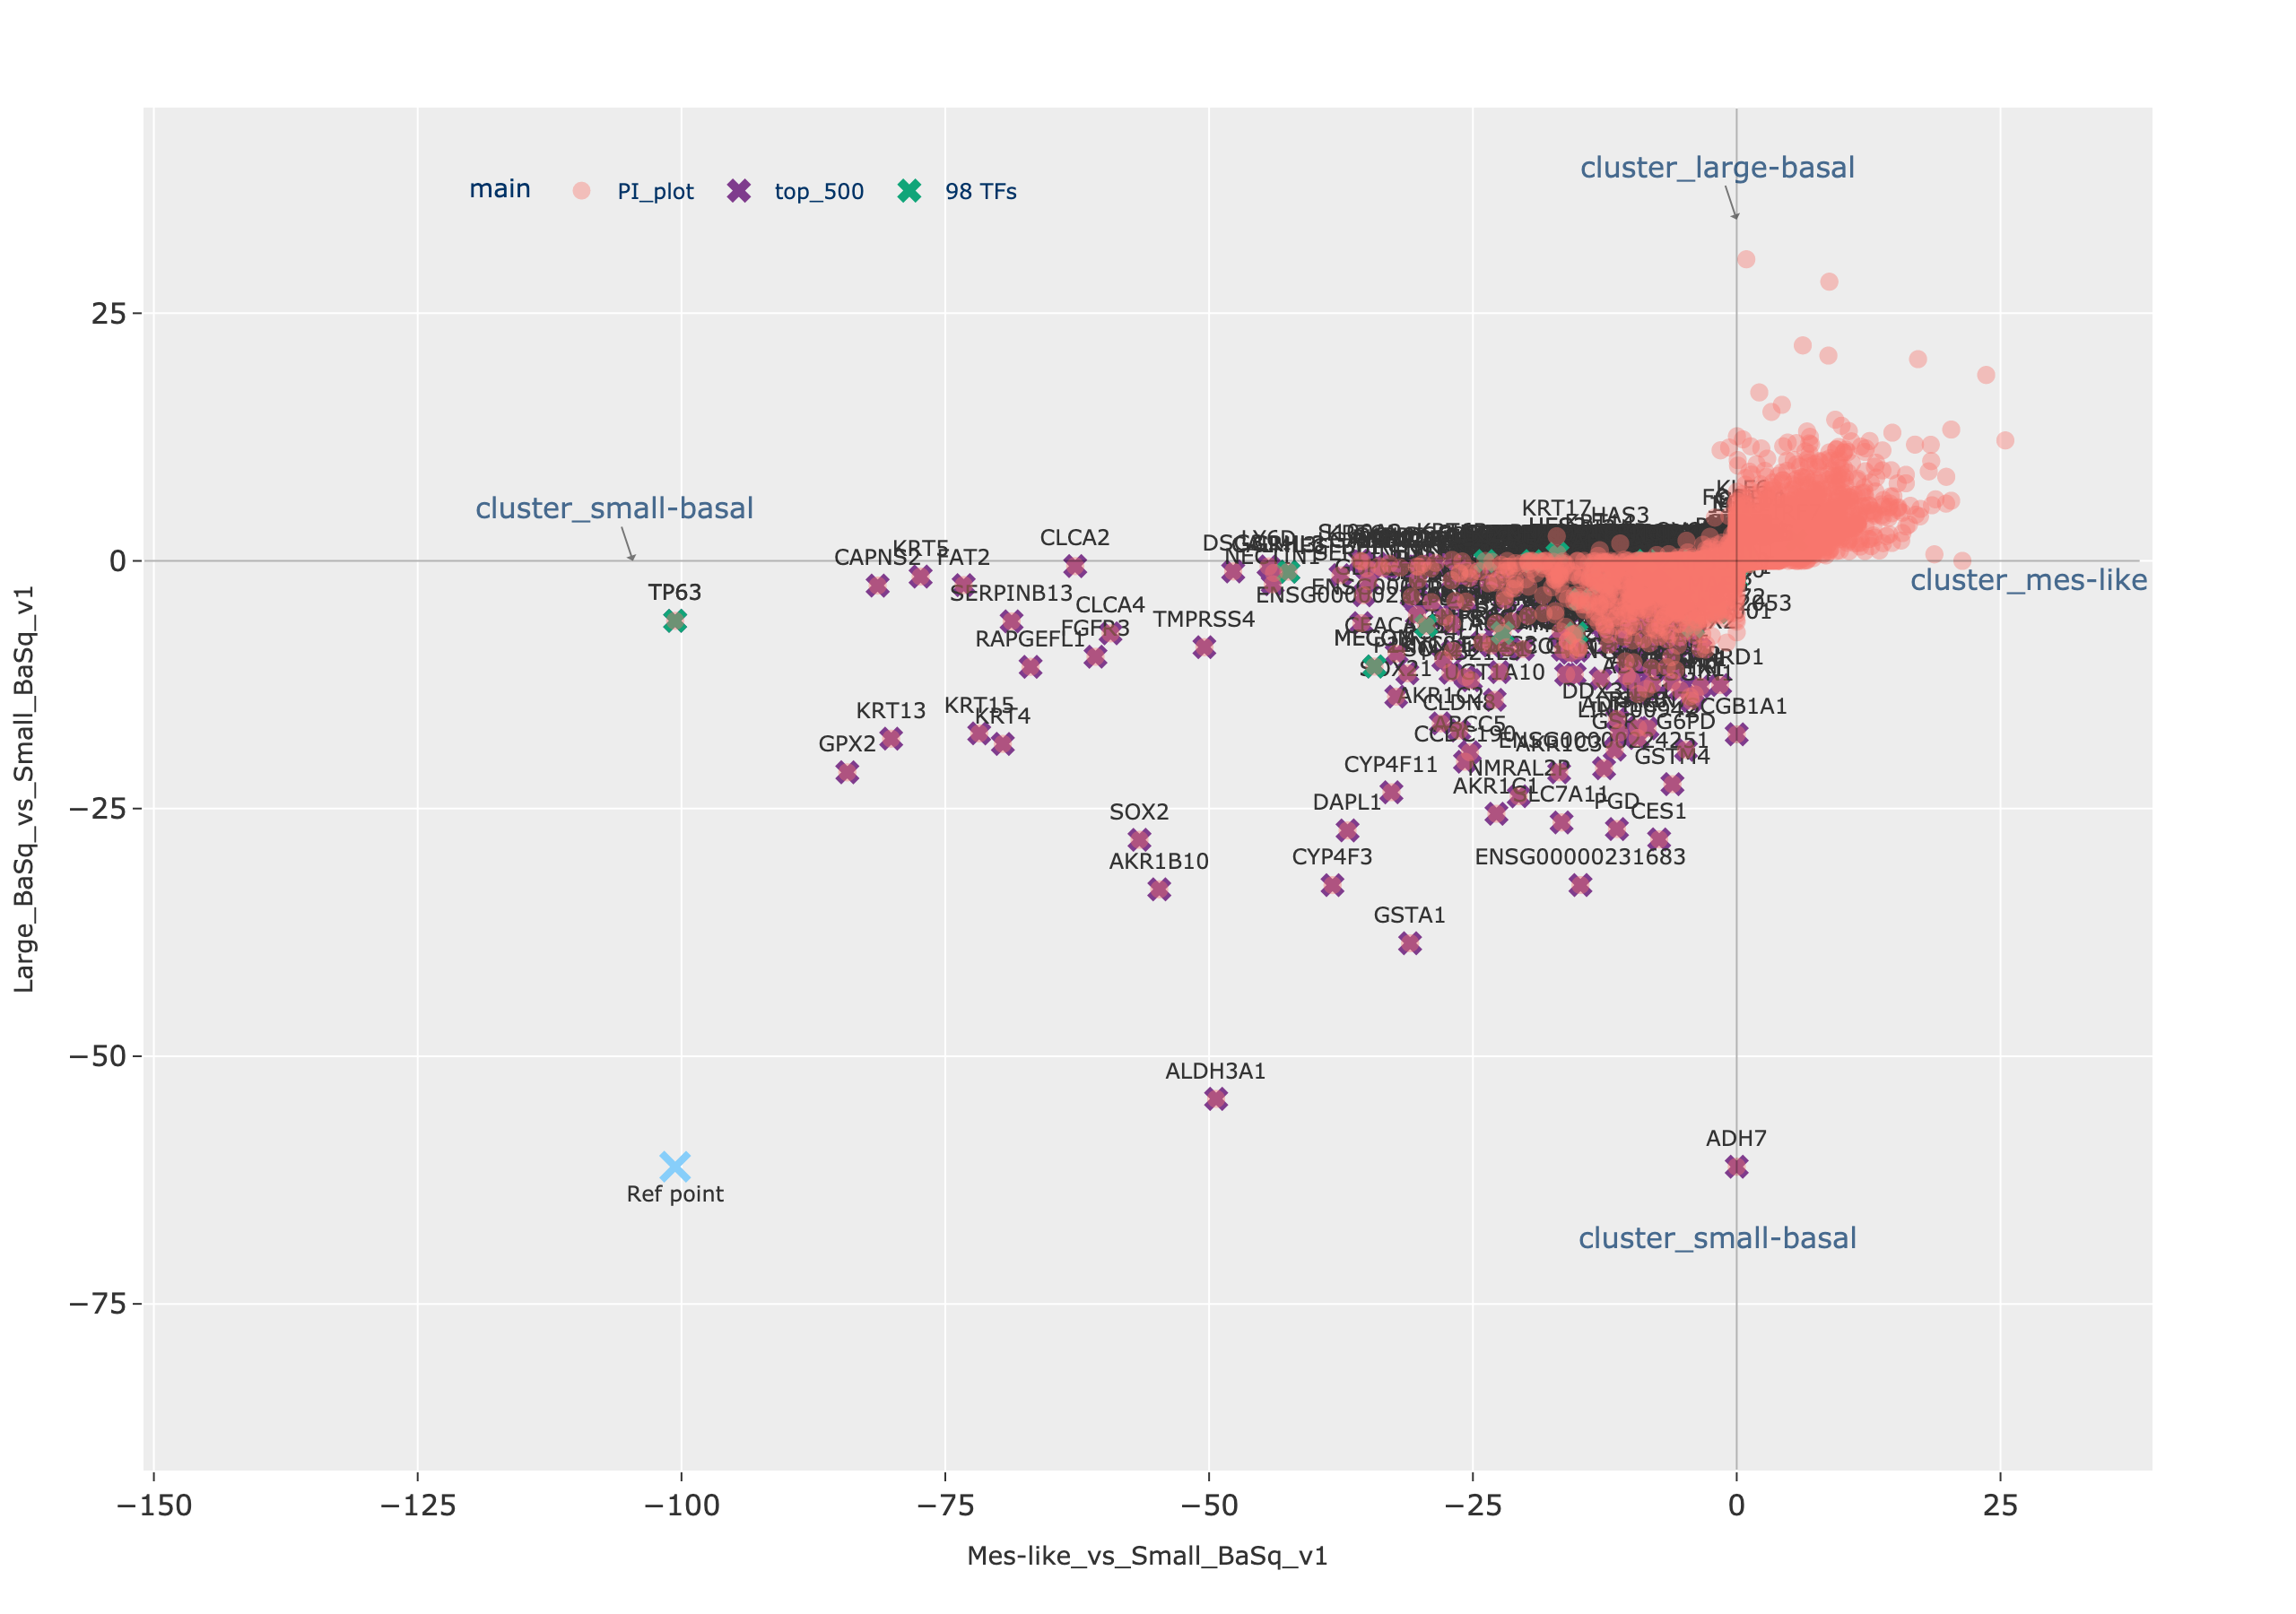
\includegraphics[width=1.0\textwidth,keepaspectratio]{Sections/Network_I/Resources/selective_pruning/pi_gsea/pi_smallBasal.png}
      \caption[Pi-plot to study the Basal group with lowest survival]{Pi plot showing the Small Basal vs Large Basal on the X-axis, and Small-Basal vs Mes-like Y-axis. This plot highlights the genes that are high and significantly expressed in the Small Basal subtype. }
    \label{fig:N_I:pi_smallBasal_comp}
\end{figure}


% Why we choose those comparisons
Basal 5 has the lowest survival prognosis seen for a subtype in this project, and to understand what differentiates it from the other groups \cref{fig:N_I:pi_smallBasal_comp} was used. The Pi-plot consists of the DEA between the Basal 4 (X-axis) and Mes 3 (Y-axis).

% 7 out of 10 biology
From the plot, it was found that seven out of the ten genes closest to the referential point were found to have biological significance in bladder cancer biology: \textit{GPX2, KRT13, ALDH3A1, KRT15, KRT4, AKR1B10, SOX2, TP53, RAPGEFL1, CAPNS2}. \textit{GPX2} is involved in squamous differentiation \citet{Naiki2018-fp}. 

% In more depth
Higher expression of \textit{KRT13} is associated with better response to chemotherapy and immunotherapy \citep{Yu2023-db}. The methylation of \textit{ALDH3A1} was studied in \gls{NMIBC} and found to be a predictor of disease recurrence \citep{McLean2023-qk}. Additionally, higher expression of \textit{ALDH3A1} in bladder cancer is associated with higher tumour grade and has been studied in cancer stem cells \citep{Kim2013-th}. \textit{KRT4} is part of the keratin family which is known to play a role in basal tumours \citep{Marzouka2018-ge}. Both \textit{AKR1B10} and \textit{SOX2} are associated with cell and cancer aggressiveness \citep{Huang2021-bn, Chiu2020-xh}, while \textit{TP53} is a known squamous marker \citep{Robertson2017-mg}. 

This evidence supports the poor survival prognosis of the smaller group and indicates that this group warrants further study. New significantly expressed genes are found such as \textit{RAPGEFL1, CAPNS2} and \textit{KRT13}.


% Small basal commenting
\paragraph*{GSEA}

The first part of table \cref{tab:N_I:gsea_basal_reactome} contains the pathways found for the small basal group which are most involved in the cell functioning. It is striking that in most of the pathways found the lead genes are matched by the 5000 genes closest to the referential point. This denotes that from the 5000 genes there are many which play an important role in multiple pathways. Disruption to the cell cycle may also explain the poor survival prognosis. 

As seen in the GSEA plot from \cref{fig:ap:gsea_smallBasal}, the enrichment score is high but not many genes are hit in the high ranked genes (i.e. top 5000) and the most hit pathways is "NFE2L2 regulating anti oxidant detoxification enzymes". The previous analysis in this section hinted that \textit{TP53} is higher expressed in the smaller group. 

% Why the top terms are kept
\subsubsection* {Basal 4}

% large basal commenting
In the second part of the \cref{tab:N_I:gsea_basal_reactome}, the pathways for the larger basal group are presented, which are mostly related to the immune response of the tissue. Especially the high match of the interferon pathways, which is expected as this groups contains the subtypes which were classified in the previous section \cref{s:clustering_analysis} as Medium IFNG and High IFNG. 


\subsubsection*{Luminal}

The table \cref{tab:N_I:gsea_luminal_reactome} contains the pathways found for the larger and infiltrated luminal subtypes. The pathway for latter mostly contains immunoglobulin related genes (e.g. \textit{IGV1-17}) denoting the infiltration of the immune cells in the bladder cancer samples. The pathways found for the large luminal are general and the lead genes have a low match ratio with the most 5000 most representative genes. This suggests that there is a less of a clear signal for a pathway to be enriched which might be explained by the size of the luminal group. 

\subsubsection*{GSEA with hallmarks}


GSEA was also applied to the hallmark gene set (50 pathways) results that can be seen in Appendix \cref{ap:tab:gsea_hallmark}. The GSEA outputs are harder to interpret due to many shared pathways but it can be observed that most of the unique pathways are found in both small basal and large luminal groups. Considering that the small basal group is considerably smaller than the large luminal, it indicates that the subtype should be study more.



% GSEA basal table (reactome)
\begin{table}[H]
  \centering
  \scriptsize
  \begin{tabularx}{\textwidth}{>{\hsize=1.9\hsize}X|>{\hsize=0.4\hsize}X|>{\hsize=0.3\hsize}X|>{\hsize=0.3\hsize}X|>{\hsize=0.5\hsize}X|>{\hsize=0.25\hsize}X}
    \toprule
    \textbf{Term} & \textbf{NES} & \textbf{FDR q-val} & \textbf{\# lead} & \textbf{\# matched} & \textbf{ratio} \\
    \midrule
    \multicolumn{6}{c}{\textbf{Basal 5}} \\
    \midrule
    NFE2L2 REGULATING ANTI OXIDANT DETOXIFICATION ENZYMES & 2.486 & 0 & 13 & 13 & 1 \\
    \midrule
    RND1 GTPASE CYCLE & 2.158 & 0 & 31 & 23 & 0.742 \\
    \midrule
    REGULATION OF RUNX1 EXPRESSION AND ACTIVITY & 2.114 & 0 & 11 & 8 & 0.727 \\
    \midrule
    SIGNALING BY PDGFR IN DISEASE & 2.101 & 0 & 13 & 9 & 0.692 \\
    \midrule
    RORA ACTIVATES GENE EXPRESSION & 2.082 & 0 & 15 & 13 & 0.867 \\
    \midrule
    GLUTATHIONE CONJUGATION & 2.063 & 0 & 20 & 17 & 0.85 \\
    \midrule
    ACYL CHAIN REMODELLING OF PC & 2.061 & 0 & 12 & 12 & 1 \\
    \midrule
    DOWNREGULATION OF ERBB2 SIGNALING & 2.034 & 0 & 14 & 14 & 1 \\
    \midrule
    SIGNALING BY ERBB2 & 2.034 & 0 & 25 & 25 & 1 \\
    \midrule
    ACTIVATION OF GENE EXPRESSION BY SREBF SREBP & 2.021 & 0 & 33 & 25 & 0.758 \\
    \midrule
    \multicolumn{6}{c}{\textbf{Basal 4}} \\
    \midrule
    INTERLEUKIN 10 SIGNALING & 2.561 & 0 & 37 & 37 & 1 \\
    \midrule
    PARASITE INFECTION & 2.545 & 0 & 89 & 84 & 0.944 \\
    \midrule
    INTERFERON ALPHA BETA SIGNALING & 2.489 & 0 & 46 & 46 & 1 \\
    \midrule
    SIGNALING BY THE B CELL RECEPTOR BCR & 2.482 & 0 & 137 & 111 & 0.81 \\
    \midrule
    FCGAMMA RECEPTOR FCGR DEPENDENT PHAGOCYTOSIS & 2.479 & 0 & 102 & 97 & 0.951 \\   
    \bottomrule
  \end{tabularx}
  \caption[Summary of the GSEA for the new basal subgroups]{Normalised Enrichment Score (NES), False Discovery Rate (FDR) q-val, and lead gene statistics for the two basal groups.The lead genes from a pathway are selected by GSEAPY based on when the NES reached its peak; see \cref{s:lit:gsea} for how GSEA was run. }
  \label{tab:N_I:gsea_basal_reactome}
\end{table}

\newpage

% GSEA luminal table (reactome)
\begin{table}[H]
  \centering
  \scriptsize
  \begin{tabularx}{\textwidth}{>{\hsize=1.9\hsize}X|>{\hsize=0.4\hsize}X|>{\hsize=0.3\hsize}X|>{\hsize=0.3\hsize}X|>{\hsize=0.5\hsize}X|>{\hsize=0.25\hsize}X}
    \toprule
    \textbf{Term} & \textbf{NES} & \textbf{FDR q-val} & \textbf{\# lead} & \textbf{\# matched} & \textbf{ratio} \\
    \midrule
    \multicolumn{6}{c}{\textbf{Lum 12}} \\
    \midrule
    SCAVENGING OF HEME FROM PLASMA & 2.396 & 0 & 54 & 47 & 0.87 \\
    \midrule
    \multicolumn{6}{c}{\textbf{Lum 13}} \\
    \midrule
    PARACETAMOL ADME & 2.016 & 0.003 & 15 & 15 & 1 \\
    \midrule
    EUKARYOTIC TRANSLATION ELONGATION & 1.864 & 0.029 & 73 & 5 & 0.068 \\
    \midrule
    SELENOAMINO ACID METABOLISM & 1.86 & 0.02 & 80 & 4 & 0.05 \\
    \midrule
    NONSENSE MEDIATED DECAY NMD & 1.832 & 0.025 & 81 & 8 & 0.099 \\
    \midrule
    SRP DEPENDENT COTRANSLATIONAL PROTEIN TARGETING TO MEMBRANE & 1.828 & 0.022 & 80 & 6 & 0.075 \\
    \midrule
    FORMATION OF WDR5 CONTAINING HISTONE MODIFYING COMPLEXES & 1.827 & 0.018 & 25 & 7 & 0.28 \\
    \midrule
    RESPONSE OF EIF2AK4 GCN2 TO AMINO ACID DEFICIENCY & 1.809 & 0.019 & 73 & 4 & 0.055 \\
    \midrule
    MITOCHONDRIAL FATTY ACID BETA OXIDATION & 1.789 & 0.023 & 28 & 18 & 0.643 \\
    \midrule
    BRANCHED CHAIN AMINO ACID CATABOLISM & 1.777 & 0.024 & 9 & 9 & 1 \\
    \midrule
    EUKARYOTIC TRANSLATION INITIATION & 1.77 & 0.025 & 76 & 5 & 0.066 \\
    \bottomrule
  \end{tabularx}
  \caption[Summary of the GSEA for the new luminal subgroups]{Normalised Enrichment Score (NES), False Discovery Rate (FDR) q-val, and lead gene statistics for the large, infiltrated and mes-like group. The lead genes from a pathway are selected by GSEAPY based on when the NES reached its peak; see \cref{s:lit:gsea} for how GSEA was run.}
  \label{tab:N_I:gsea_luminal_reactome}
\end{table}


\newpage

% Metadata exploration
\subsection{TCGA metadata exploration} \label{s:N_I:sel_tfs_metadata}

To understand better the biology of the small basal group, the metadata from TCGA \citep{Cancer_Genome_Atlas_Research_Network2014-xp} was used. Several features were explored: level of smoking (cigarettes per day), race, metastasis, relation to noninvasive bladder cancer, and histology grade. \Cref{fig:ap:sel_tfs_tcga_metadata} from Appendix displays this information in the form of multiple histograms, where the x-axes represent the subtypes derived in this section and the y-axes the count of the metadata features. From the figure, there is no immediate characteristic for the small basal group, neither with the Squamous pathology nor with the metastatic status, but most of the patients were smokers. It is worth pointing out that LumInf, Mes-like, and large luminal groups are generally characterised by non-squamous tumours. 

From the appendix \Cref{fig:ap:sel_tfs_tcga_meta_mut} shows that there is no immediate relationship with the mutations selected in the TCGA supplementary material.


% Linking to communities
\subsection{Linking back to the communities} \label{s:N_I:sel_tfs_net}

% Network stats
To leverage visualising aspect of the network, the basal/luminal markers were then searched in the experiment 5000 genes network generated using no weight modifiers (standard), minimum 3 edges per genes and 6 for the TF, and to which the Stochastic Block Model was applied. Neither of the markers, basal/luminal or for differentiated, were not grouped in a single or 2-3 communities, but rather spread across several.


\begin{figure}[!t]
    \centering
    \begin{subfigure}[!t]{0.49\textwidth}
        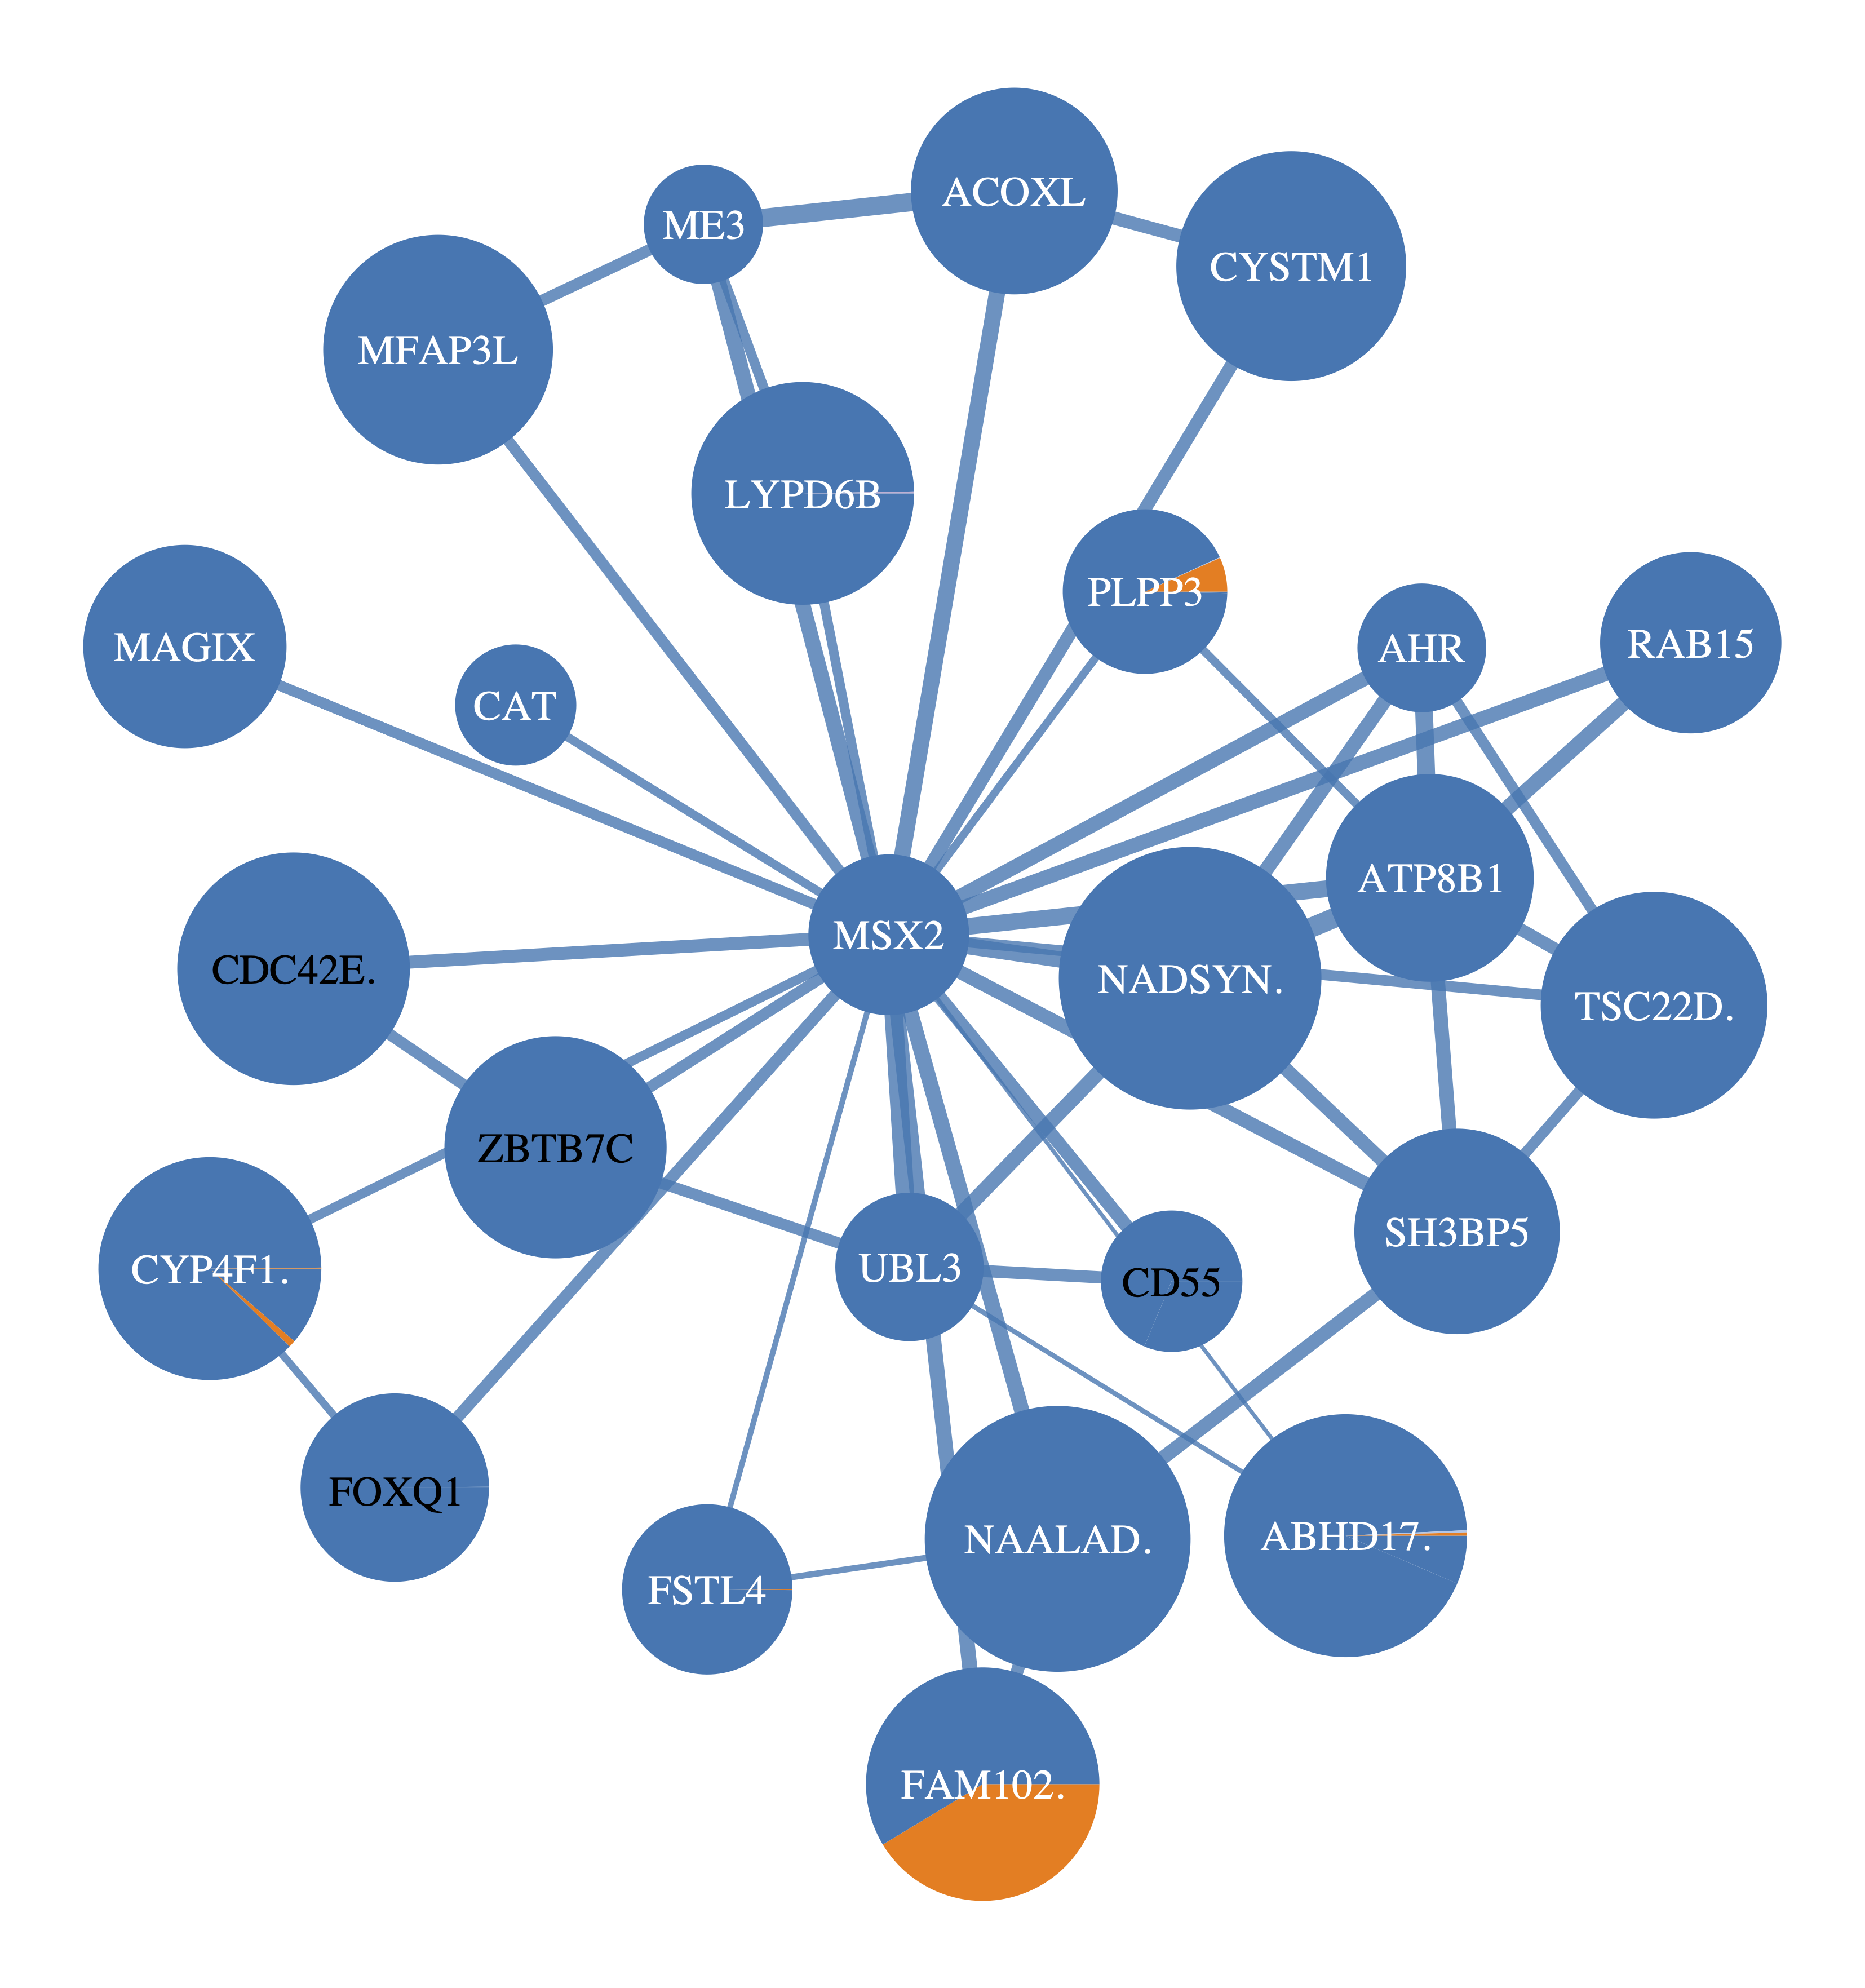
\includegraphics[width=1.0\textwidth,height=1.0\textheight,keepaspectratio]{Sections/Network_I/Resources/selective_pruning/net/net_MSX2.png}
        \caption{\textit{MSX2} (luminal)}
        \label{fig:N_I:net_MSX2}
    \end{subfigure}
    \centering
    \begin{subfigure}[!t]{0.49\textwidth}
        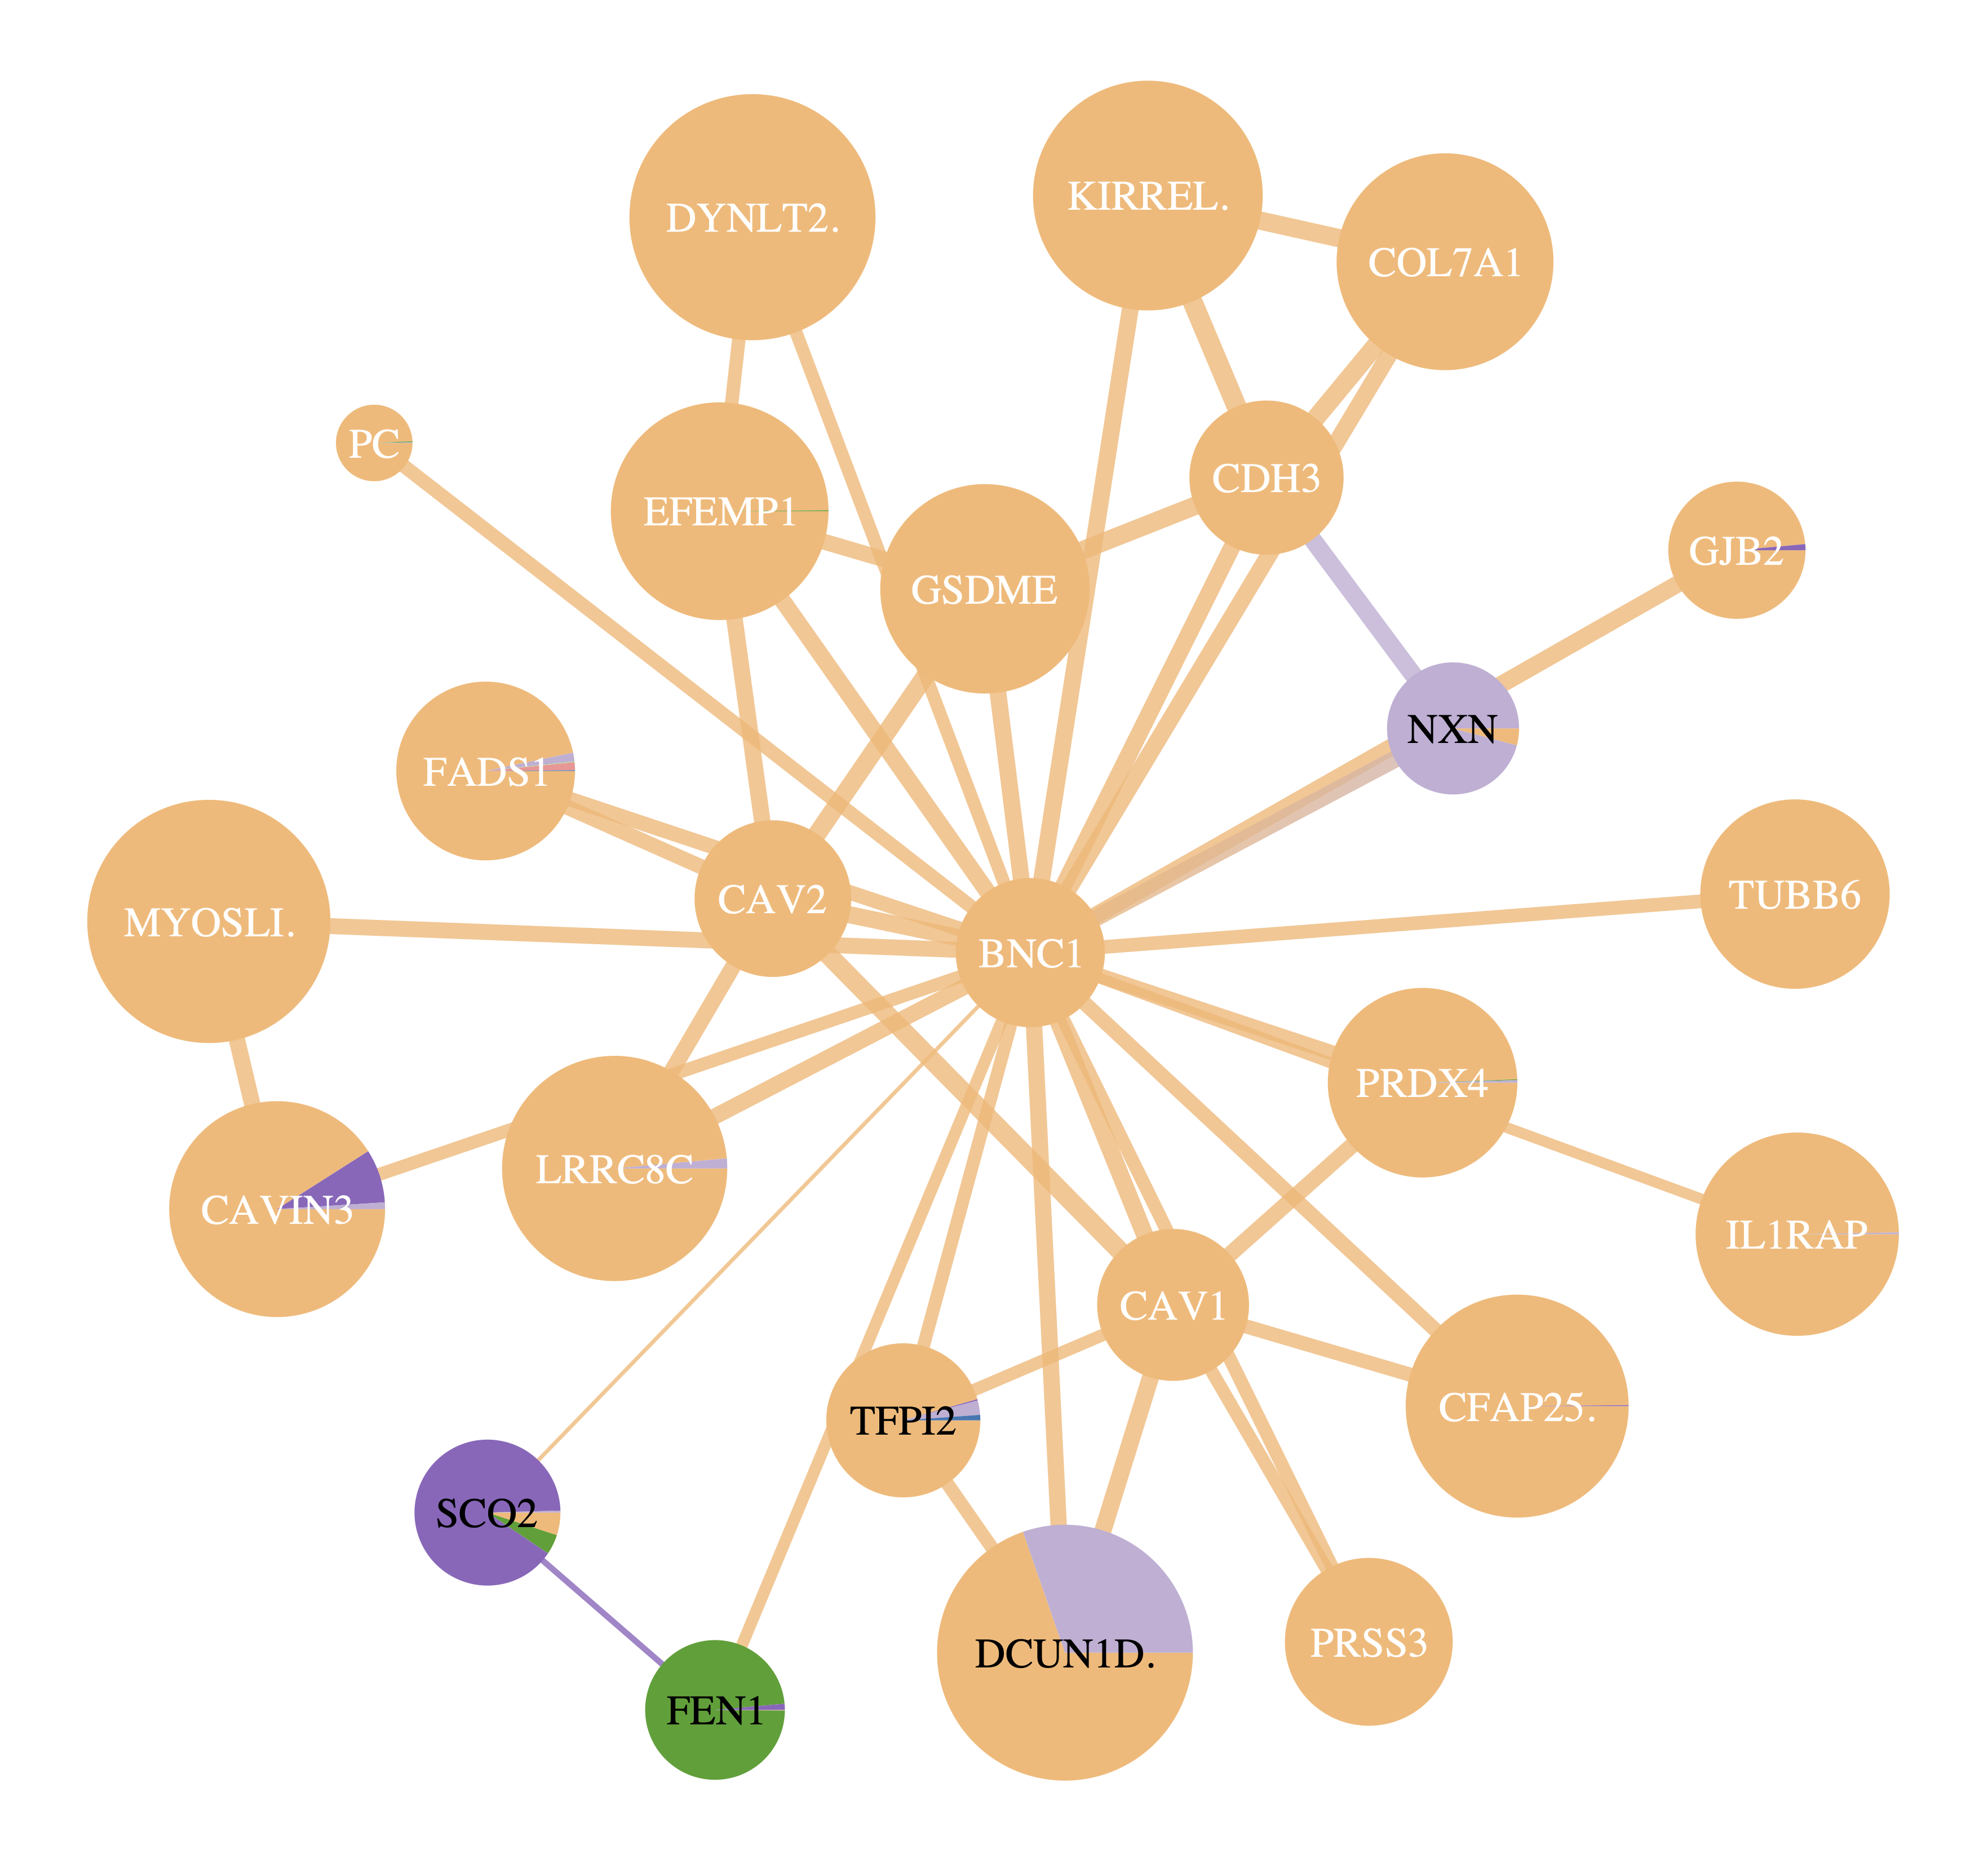
\includegraphics[width=1.0\textwidth,height=1.0\textheight,keepaspectratio]{Sections/Network_I/Resources/selective_pruning/net/net_BNC1.png}
        \caption{\textit{BNC1} (basal)}
        \label{fig:N_I:net_BNC1}
    \end{subfigure}
    \caption[Network neighbours of \textit{MSX2} and \textit{BNC1}]{The \textit{MSX2} luminal and \textit{BNC1} markers and their neighbours in a standard network (no weight modifier), where a minimum of 6 edges are allowed per TF and the Stochastic Block Model was applied to detect the communities. The size of the nodes is proportional to the degree of the gene and the edge weight to the correlation value.}
    
    \label{fig:N_I:net_neighbours}
\end{figure}

% Neighbours 
When filtering the network to display the neighbours of a  gene from the basal/luminal markers, it is often the case that markers are linked together, meaning that are co-expressed. \Cref{fig:N_I:net_MSX2} shows the sub-graph for \textit{MSX2} in which other markers such as \textit{FOXQ1, ZBTB7C} are linked directly to the gene. \textit{AHR} is also connected to \textit{MSX2}. \textit{AHR} has been extensively studies in the bladder cancer, urothelium and it is highly mutated in the TCGA cohort. It is also studied in more depth in the next chapter \ref{s:N_II}. In the sub-network for \textit{BNC1} , \cref{fig:N_I:net_BNC1}, there are less known genes but \textit{CDH3} is a basal marker \citep{Dadhania2016-cb} and \textit{CAV1, CAV2}. 

It is worth noting that both genes, have considerable more than 6 neighbours. This suggests that there are many genes that have either \textit{BNC1} or \textit{MSX2} in their top correlated values. The kind of visualisation in \cref{fig:N_I:net_neighbours} is useful to narrow down the search for targets and potential co-expressed genes.


Therefore, the 98 transcription factors and the two lists of Ba/Sq and Luminal markers are validated by research from different groups. The expression of these genes across the MIBC, from both the consensus and the subtypes derived from hierarchical clustering, can be seen in \cref{fig:N_I:box_debdrogram}. This also serves as an encouragement to explore the other genes not matched by other research, as they may exhibit potential for new biological insights.


